%!TEX TS-program = xelatex
%!TEX encoding = UTF-8 Unicode
\documentclass[handout]{beamer}
\usetheme{CambridgeUS} % replace it with Boadilla if you want no section bar
%\usecolortheme{crane} % other ones: dove, dolphin, rose, seahorse, orchid, crane, seagull, lily, wolverine
%\usefonttheme{serif} 
\usefonttheme[onlymath]{serif} % uncomment if you want it just for math

\setbeamertemplate{navigation symbols}{}  % comment to have nagivation

\usepackage[compress,comma,authoryear]{natbib}
\usepackage{tikz}
\usetikzlibrary{mindmap,trees}
\usepackage{amsmath,mathtools}
\usepackage{amsthm}
\usepackage{booktabs}
\usepackage{graphicx,epstopdf}
\usepackage{hyperref}

\usepackage{fontspec}
\newfontfamily{\FA}{XB Niloofar}[Extension = .ttf] % Farsi
\newfontfamily{\FAN}{IranNastaliq}[Extension = .ttf] % Farsi Nastaliq

\definecolor{blue}{RGB}{0,114,178}
\definecolor{red}{RGB}{213,94,0}
\definecolor{yellow}{RGB}{240,228,66}
\definecolor{green}{RGB}{0,158,115}
\definecolor{Lblue}{RGB}{0,197,155}
\definecolor{Dblue}{RGB}{0,76,119}
\definecolor{Lgreen}{RGB}{180,255,230}

\hypersetup{
	colorlinks=false,
	linkbordercolor = {white},
	linkcolor = {blue}
}
\definecolor{MyBackground}{RGB}{245,245,245}

\setbeamercolor{frametitle}{fg=blue}
\setbeamercolor{title}{fg=blue}
\setbeamertemplate{footline}[frame number]
\setbeamertemplate{navigation symbols}{} 
\setbeamertemplate{itemize item}[circle]%{$\bigstar$}
\setbeamertemplate{itemize subitem}{$\bigstar$}
\setbeamercolor{itemize item}{fg=blue}
\setbeamercolor{itemize subitem}{fg=blue}
\setbeamercolor{enumerate item}{fg=blue}
\setbeamercolor{enumerate subitem}{fg=blue}
\setbeamercolor{button}{bg=MyBackground,fg=blue}
\setbeamercolor*{palette primary}{use=structure,fg=blue,bg=white}
\setbeamercolor*{palette secondary}{use=structure,fg=white,bg=Dblue}
\setbeamercolor*{palette tertiary}{use=structure,fg=white,bg=blue}
\setbeamercolor*{palette quaternary}{fg=white,bg=black}
\setbeamercolor*{palettes quaternary}{fg=white,bg=Lgreen}
%\setbeamercolor{titlelike}{parent=structure,bg=Lgreen}
%\setbeamercolor{title in head/foot}{bg=Lgreen,fg=orange}

\setbeamertemplate{enumerate item}{%
	\usebeamercolor[bg]{item projected}%
	\raisebox{1.5pt}{\colorbox{blue}{\color{fg}\footnotesize\insertenumlabel}}%
}



\begin{document}
	\title[Econometrics 2]{Econometrics 2 (M.Sc.)}
	\subtitle{Introduction}
	\author[Mohammad Hoseini]{Mohammad Hoseini}
	
	%\institute[IMPS]{Institute for Management and Planning Studies (IMPS)}
	
	\date[Spring 2025]{Spring 2025 \\
		 \vspace{10pt} @metrics2
	}
	
\begin{frame}[plain]
	\titlepage
\end{frame}

\section{Preliminaries }
\subsection{Introduction}

\begin{frame}{Introduction}
In this course, we aim at improving your understanding about empirical research in economics and teaching you how to apply the econometrics methods. \medskip

%We try to make you enjoy econometrics \url{https://www.youtube.com/watch?v=WwW8y5dZs80}\bigskip
%\begin{center}
%	{\FA \LARGE میان \ به \ آید \ تجربه \ محک \ گر \ بود \ خوش}
%\end{center}

At the end of the course, you are expected to learn:

\begin{enumerate}
	\item Learning some techniques
	\begin{itemize}
		\item Learning different techniques are important but not enough to be good empirical economist. You must also ask interesting research questions.
	\end{itemize}	
	
	\item Finding a good \textbf{identification strategy} to answer them.
	\begin{itemize}
	\item On the other hand, you might have a great idea, but if your identification strategy and empirical analysis is poor the research project fails.
	\end{itemize}

\end{enumerate}

\end{frame}



\subsection{Data types}

\begin{frame}{The evolution of data types and econometrics}
Before 1970s:
\begin{itemize}
\item Data type: aggregate macro variables
\item Methods: linear cross-country regressions, early time series
\end{itemize}\bigskip\pause

1970s  to early 2000s:
\begin{itemize}
	\item Data type: representative household/firm surveys
	\item Methods: microeconometrics, non-linear models, panel data, quasi-experiments, structural models
\end{itemize}\bigskip

New trends:
\begin{itemize}
	\item Data types: big data / randomized experiments
	\item Methods: AI, less assumption on distribution
\end{itemize}
\end{frame}

\begin{frame}{Econometrics: the path from cause to effect}
	What is the difference between statistics and econometrics?\bigskip
	
	What is the difference between data science and econometrics?\bigskip
	
	Do we need to learn econometrics when machine learning method can make good prediction?\bigskip
	
	Let's watch some videos from Josh Angrist (noble laureate 2022) 
	\begin{itemize}
		%\item \url{https://www.youtube.com/watch?v=WwW8y5dZs80}
		\item \url{https://www.youtube.com/watch?v=uVrr_-UUgWk}
		\item \url{https://www.youtube.com/watch?v=2EhRT2mOXm8}
		\item \url{https://www.youtube.com/watch?v=Bm6CAjVtrIw}
	\end{itemize}

\end{frame}


\begin{frame}{This course}
Type of data:

\begin{itemize}
	\item Level: individuals, firm, household, and sometime region and state
	\item Time: cross-section, panel (longitudinal), repeated cross-section
	\item Randomness: observational, experimental
\end{itemize}\bigskip\pause


Objectives:
\begin{itemize}
	\item Data mining: summary statistics, correlation tables, simple regressions
	\item \textbf{Causal inference}: testing and measuring a theory
\end{itemize}

\end{frame}


\begin{frame}{Randomness of micro data}
Observational data:

\begin{itemize}
	\item Census and survey data
	\item Administrative data
	\item Transaction data
	\item Internet data
\end{itemize}\bigskip

Experimental data:
\begin{itemize}
	\item The assignment of the treatment is monitored.
	\item Possible to vary the causal variable of interest while controlling for other covariates.
\end{itemize}
\end{frame}

\begin{frame}{Type of observational data:}
\textbf{Cross-section}: a snapshot of characteristics of many units like one-shot surveys.\bigskip

\textbf{Time-series}: the characteristics of a single unit over time\bigskip

\textbf{Repeated cross-section}: Same questionnaire surveyed overtime each time for a new random sample e.g. annual household surveys. Good for making a representative sample of the whole population over time.\bigskip

\textbf{Panel or longitudinal}: Survey of same units over time. Good for tracking unit-based changes.\bigskip

\textbf{Rotated panels}: a subset of units are sampled overtime. Making a representative sample while tracking changes for some units.\bigskip

\textbf{Pseudo-panels}: aggregating repeated cross-section into representative units which are constant overtime. For example making state-level unemployment rate over time using annual surveys.
\end{frame}


\begin{frame}{Survey data}
Representative (random sampling) and non-random (online surveys)\bigskip

Simple random sampling: the probability of sampling each unit from a population of size $N$ is $1/N$.\bigskip

Multistage surveys: All nation-wide surveys are based on multistage sampling.  \bigskip

Each stage of the sampling consist of mutually exclusive subsets of population 
\begin{itemize}
	\item Strata like province or state, 
	\item Primary units like districts within a state, 
	\item Secondary units like cities or villages,
	\item Ultimate sampling units like different zones within a city
\end{itemize}

As a result, the probability of sampling is changing for different units.\medskip

In this case, we MUST use sample weight (multiplier) which is the inverse of the probability of sampling. 

\end{frame}

\begin{frame}
	\begin{center}
		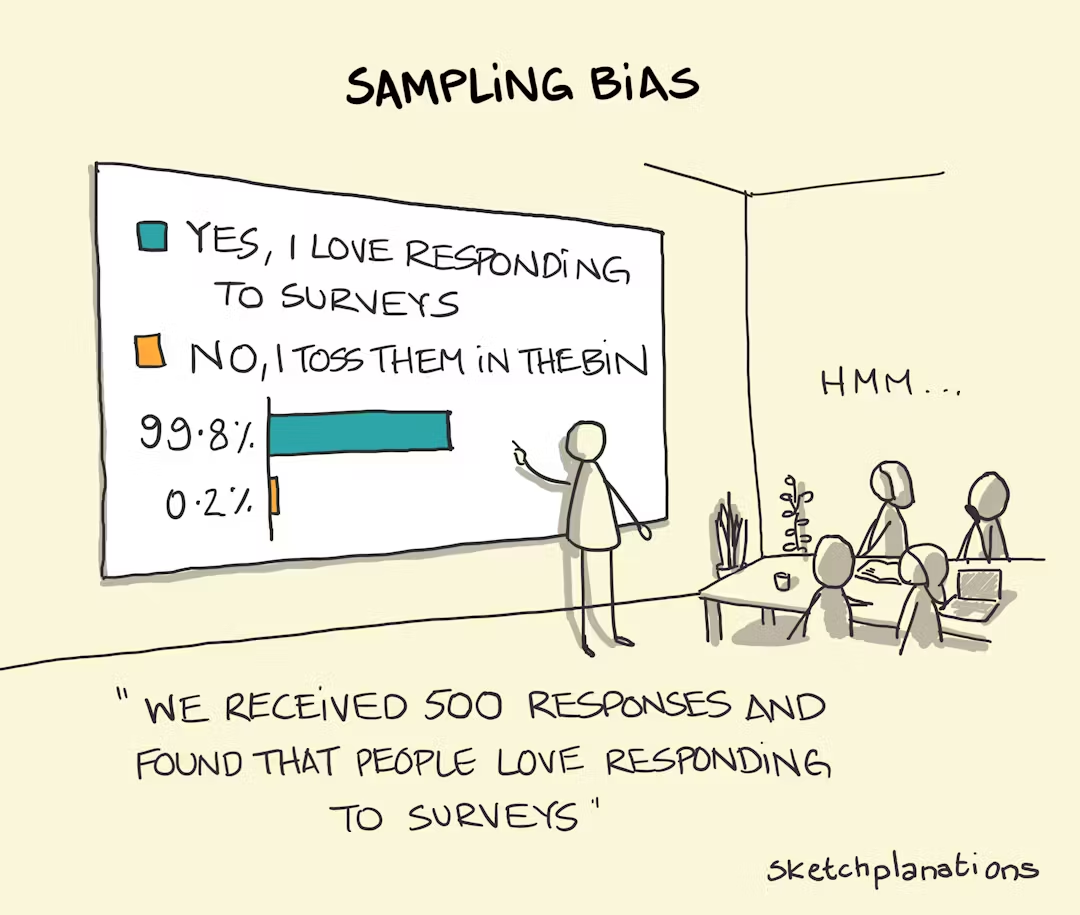
\includegraphics[width=0.9\linewidth]{./Figures/Sampling_bias.png}
	\end{center}
\end{frame}



\begin{frame}{Common problem in surveys}
Nonresponse: if it is in a systematic manner the randomness may be violated.\bigskip

Missing data\bigskip

Measurement error: respondent might misreport deliberately or do not recall precisely or do not understand the question correctly.\bigskip

Sample attrition in longitudinal data

\end{frame}


\begin{frame}{Popular surveys in Iran}
Census of Population and Housing ({\FA مسکن و نفوس عمومی سرشماری})
\begin{itemize}
	\item decennial in 1956-2006, 2011, 2016
\end{itemize}\bigskip

%Employment and Unemployment Survey (1997-2004):
%\begin{itemize}
%	\item Problems in sample weights
%	\item Raw data is not distributed
%\end{itemize}\bigskip

Labor force survey ({\FA کار نیروی طرح})
\begin{itemize}
	\item Quarterly (around 150,000 individuals) since 1384
	\item Rotated panel: each household is sampled in two consecutive seasons and in two consecutive years. 
	\item Every four years the panel is entirely refreshed.
	\item Not seasonal in all years.
\end{itemize}

\end{frame}

\begin{frame}{Popular surveys in Iran}
Household Income and Expenditure surveys ({\FA خانوار درآمد و هزینه طرح})
\begin{itemize}
\item Yearly (around 50,000 household)
\item Rotated panel after 2010 (1989)
\item A detailed questionnaire around 70 pages on various expenditure items
\item Brief information about income
\end{itemize}\bigskip

{Firm-level surveys}
\begin{itemize}
\item Annual Survey of Industries ({\FA صنعتی کارگاه‌های})
\item Service sector surveys ({\FA خدمات و بازرگانی طرح})
\end{itemize}

\end{frame}


\subsection{Reproducibility}

\begin{frame}{Research must be reproducible}

Theory can be checked by mathematics.\bigskip

But you should learn to do ``reproducible'' empirical research as well.

\begin{itemize}
	\item Others can easily repeat the findings using data and codes
	\begin{itemize}
		\item Different from replication: same conclusion in a new study
	\end{itemize}
	\item No copy-paste, no GUI use, document everything you do in codes
\end{itemize}\bigskip

Different stages of empirical research:\medskip

Raw data $\Rightarrow$ clean $\Rightarrow$ transform $\Rightarrow$ summarize $\Rightarrow$ analyze $\Rightarrow$ report\bigskip

New standard for economic journals: \url{https://datacodestandard.org/}
\end{frame}

\begin{frame}{Example: effect of SEZ on unemployment}
You want to study the impact of becoming a Special Economic Zone on unemployment rate of a city using census data.
\begin{itemize}
	\item Raw data: Obtain census data in the raw format.
	\item Clean: import raw data-files of census, merge the needed data files, drop unused variables and outliers, generate new variables.
	\item Transform: aggregate the cleaned household data to city-level.
	\item Summarize: show stylized facts by a map, time-series graph, summary tables, etc.
	\item Analyze: regress unemployment on SEZ and proper control variables.
	\item Report: export the results and interpret.
\end{itemize}

\end{frame}


\begin{frame}{Software}
You can use lots of softwares. Empirical economist normally use STATA and R.\bigskip
%\begin{figure}
%	\centering
%	
\includegraphics[width=0.7\linewidth]{../figure/software.jpg}
%\end{figure}

Graphical user interface (GUI) is available for Stata \& R (Rstudio) and other softwares, but we want everything coded.\medskip

%The general rules are the same in other softwares.\bigskip

Important things to remember:
\begin{itemize}
	\item file structuring
	\item clean coding
	\item variable naming and labeling
\end{itemize}
\end{frame}

%\begin{frame}{R vs STATA}
%\begin{tabular}{p{.475\textwidth}|p{.475\textwidth}}
%	R	& STATA\\
%	\hline
%	open source	& expensive \\
%	closer to data science (stats / machine learning) commiunity	& closer to econometricans \\
%	package loading structure &	no hassle, much simpler syntax and module download \\
%	powerfull visualization (ggplot2)&	simpler visualization \\ 
%	can import many files&	supports much less formats \\
%	poor support of Farsi&	much poorer in Farsi! \\
%	Poor help many online resources&	better standard help \\
%	support of Latex and better reproducibility&	great GUI \\
%	easier writing of programs& shared standard among economists \\
%	work much better with big data	&\\
%\end{tabular}

%\end{frame}

\begin{frame}{File structuring}
\begin{columns}
	\begin{column}{.3\textwidth}
Separate out data, codes, output in folders.\bigskip

Split long codes to multiple script files.\bigskip

Place a 'Read me' file in the main folder and explain the details.
	\end{column}
	\begin{column}{.7\textwidth}
	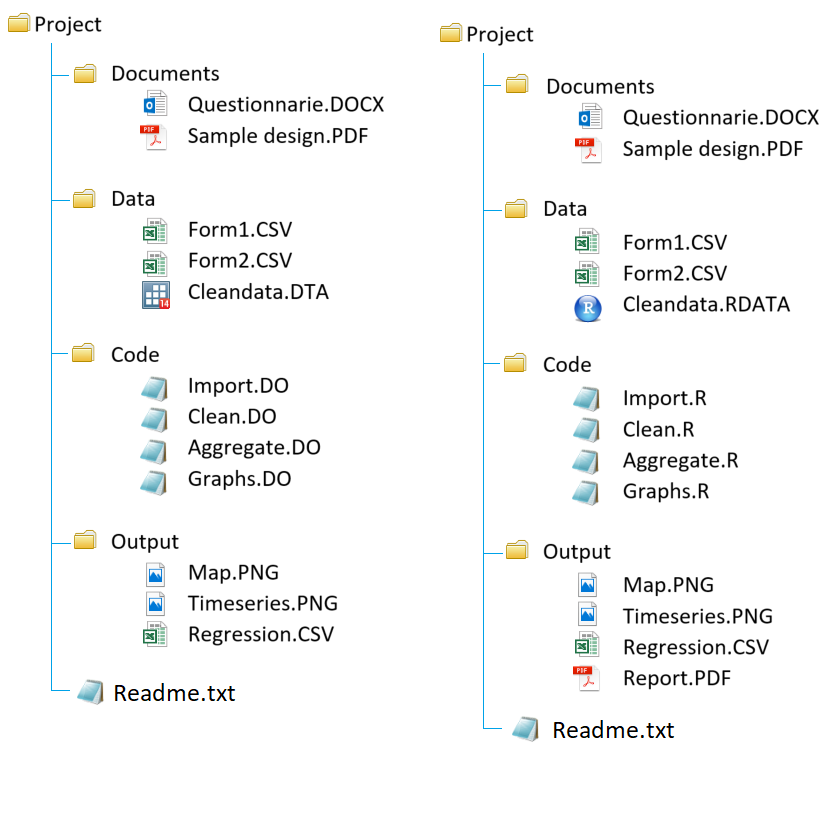
\includegraphics[width=\textwidth]{./Figures/filestructuring}
	\end{column}
\end{columns}
\end{frame}

\begin{frame}{Coding}
Which one is more understandable?\bigskip

	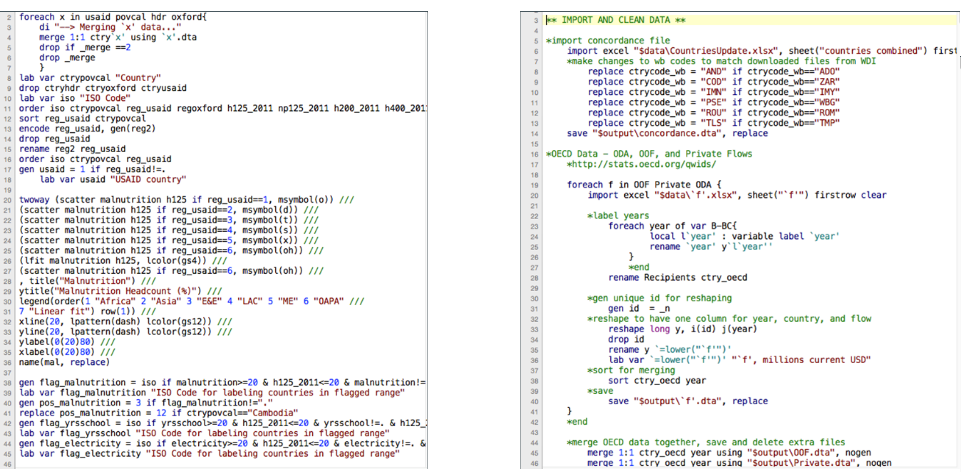
\includegraphics[width=\textwidth]{./Figures/coding}
\end{frame}


\begin{frame}{Naming}
Names are case-sensitive.
\begin{itemize}
	\item ideally, the names are short but clear ( better to be clear than short).
	\item stick to a naming convention that is intuitive and consistent across your projects.
	\item generally, function names are usually verbs, and variables are nouns.
	\item in STATA you can describe the variables using 'label var' command.
\end{itemize}
\end{frame}



\begin{frame}{Outline}
	\begin{columns}
		\begin{column}{.5\textwidth}
			\textbf{Part 1: Methods}
			\begin{itemize}
				\item Recap of OLS
				\item Maximum likelihood (MLL)
				\item Generalized method of moments (GMM)
				\item Binary response models (probit/logit)
				\item Panel data estimation
			\end{itemize}
		\end{column}
		\begin{column}{.5\textwidth}
			\textbf{Part 2: Causal inference}
			\begin{itemize}
				\item Selection bias \& experiments
				\item Conditional independence assumption
				\item Matching
				\item Instrumental variables
				\item Difference in difference
				\item Regression discontinuity design
			\end{itemize}
		\end{column}
	\end{columns}	
\end{frame}

\begin{frame}{Suggested textbooks}
Cunnningham (2021), \textbf{Causal inference: The mixtape}
	\begin{itemize}
		\item a practical book with R and STATA examples
	\end{itemize}\medskip

Cameron and Trivedi (2005), \textbf{Microeconometrics: Methods and Applications}
\begin{itemize}
	\item Good for first part of the course MLL, GMM, panel data
\end{itemize}\medskip

Imbens and Rubin (2015), \textbf{Causal inference} %for statistics, social, and biomedical sciences
\begin{itemize}
	\item a more technical book for the second part of the course
\end{itemize}\medskip

		
		Lee (2016) \textbf{Matching, Regression Discontinuity, Difference in Differences, and Beyond}\bigskip
		
		Angrist and Pischke (2009) \textbf{Mostly Harmless Econometrics}

\medskip
\end{frame}


\begin{frame}{Logistics}
	\begin{columns}
		\begin{column}{0.7\textwidth}
			Grading: 
			\begin{itemize}
				\item exams (12 points),
				\item exercises (8 points), 
				\item class participation can have extra grade.
			\end{itemize}\medskip
			
			Attendance Policy: 
			\begin{itemize}
				\item If you miss more than 3 classes, every additional absence will lower your class grade by 1 points. With more than 5 absences, you will fail the course.
			\end{itemize}
	\end{column}
	\begin{column}{0.3\textwidth}\begin{center}
			Office hours:
		\end{center}
	
\includegraphics[width=\textwidth]{./Figures/qrcode}
	\end{column}
	\end{columns}\begin{flushright}\url{https://calendly.com/hoseini} \end{flushright}
	 



	%TA sessions: Wednesdays 10:00-12:00\medskip

\end{frame}


\begin{frame}{TAs}
%\textbf{Exercises:} \medskip
\begin{center}
%\includegraphics[width=.35\textwidth]{./Figures/Younes}\qquad\qquad
%	\includegraphics[width=.35\textwidth]{./Figures/iranpur}
	
{\FAN\LARGE حیدری \ \ یونس}\qquad\qquad\qquad\qquad\qquad\qquad  {\FAN\LARGE ایران‌پور \ \ علی}
\end{center}\bigskip	

\end{frame}




\end{document}
